\documentclass{article}
\usepackage[utf8]{inputenc}
\usepackage[ukrainian]{babel}
\PassOptionsToPackage{hyphens}{url}\usepackage{hyperref}
\title{Прикладні алгоритми. Завдання 2, Bug Report}
\author{Михайло Голуб}
\usepackage{graphicx}
\graphicspath{ {./images/} }
\begin{document}
\maketitle
\newpage

\textbf{Як було виявлено проблему:}\\\indent
Під час виконання четвертого завдання для реалізації алгоритму Крускала було обрано варіант реалізації де необхідно відсортувати усі ребра за вагою. Для перевірки правильності сортування в консоль було виведено відсортований масив трійок вершина-вершина-вага, що описують ребра. В даному масиві було забагато однакових значень ваги.\indent

Для кращого розуміння проблеми, було виведено повну матрицю суміжності в консоль. В усіх випадково згенерованих графах рядки таблиці містили або відсутність значення, або однакове значення. Це призводило до того що згенерований граф виходив майже зажди орієнтований і з вершин, з яких виходило хоча б одне ребро, виходили всі можливі ребра. \\\\\indent

\textbf{Пошук джерела проблеми:}\\\indent
Було перевірено кожен крок зміни матриці починаючи з останнього. Перевірками було виявлено що кількість записів змін співпадає з очікуваною кількістю, але кількість змінених значень перевищує очікування. Одразу було створено гіпотезу щодо неправильного створення пустої матриці суміжності: усі елементи рядків матриці виявились вказівниками на один об'єкт, а не на різні.\\\\\indent

\textbf{Вирішення проблеми:}\\\indent
Створення пустої матриці суміжності замінено з "добутку" рядків на з'єднання копій рядків.\\\\\indent

\textbf{Додаткові зміни:}\\\indent
Для простоти роботи з методами класів, відсутність ребра у зважених графів перепозначено з False на None, оскільки 0 == False.\\\\\indent

\textbf{Вплив виправлення проблеми на результати тестів часу роботи методів:}
Виправлення проблеми не вплинуло на швидкість роботи методів додання та видалення ребер і вершин. Це очікувано, оскільки це операції зміни однієї або двох клітинок матриці.\\\indent
 Виправлення проблеми призвело до правильної побудови графів і тепер алгоритми перетворення матриці на списки суміжності та навпаки, складність яких залежить від кількості ребер, мають працювати правильно і їх складність тепер має збігатись з теоретичною O(n), де n -- кількість ребер.

Результати тестування \textit{add\_edge}:
\begin{center}
    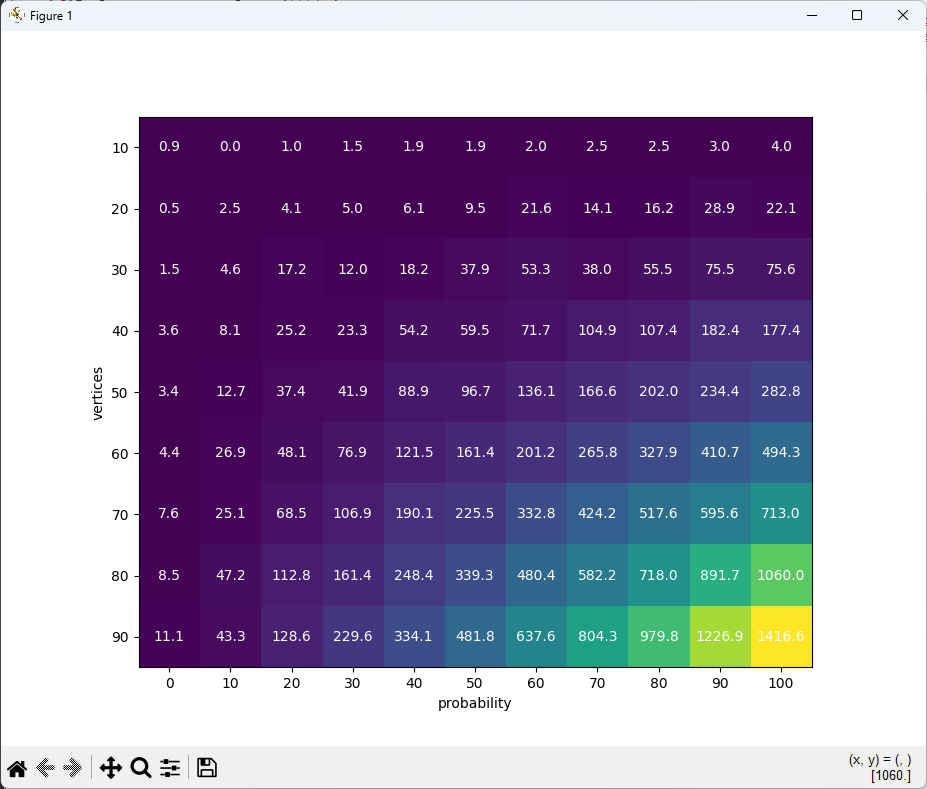
\includegraphics[width=125mm]{newtoll}
\end{center}\indent

З нової теплової мапи часу роботи перетворення матриці суміжності на списки видно, що: залежність часу роботи від імовірності створення ребра є лінійною; залежність часу роботи від кількості вершин є експоненційною. Якщо об'єднати ці залежності, вийде лінійна залежність часу роботи від кількості ребер. Це збігається з теоретичною оцінкою.

\begin{center}
    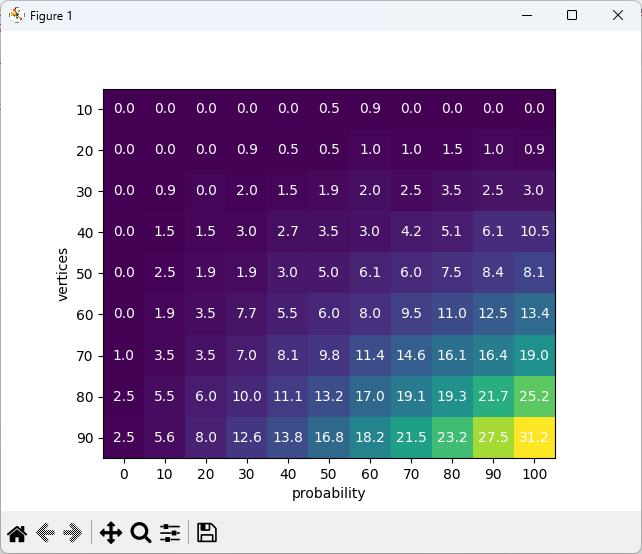
\includegraphics[width=125mm]{newfromll}
\end{center}\indent

З нової теплової мапи часу роботи створення матриці суміжності зі списків видно, що: залежність часу роботи від імовірності створення ребра є лінійною; залежність часу роботи від кількості вершин є експоненційною. Якщо об'єднати ці залежності, вийде лінійна залежність часу роботи від кількості ребер. Це збігається з теоретичною оцінкою.



\end{document}